% !TeX root = ../../../master.tex

\subsection{Benutzerkonto}
\label{ssec:Benutzerkonto}

Jeder Nutzer erhält die Möglichkeit sein eigenes Passwort zu ändern, was als Funktion im Benutzerkonto eingebunden ist.
Zum Benutzerkonto gelangt der Benutzer über das Icon \faUser[regular]\xspace in der Navigationsleiste.
Abbildung~\myRefGeneral{fig:AccountImplement} zeigt dabei beispielhaft ein Benutzerkonto.
Das Passwort kann nun über die eigene Account-Karte geändert werden, wodurch die Anforderung~\hyperref[Anf:A4]{A4}, die Möglichkeit zur Passwortänderung, erfüllt wird.

Zudem kann der Nutzer über den Knopf \jinline|Show Published Surveys| der zweiten Karte auf das Result-Dashboard navigieren (siehe Kapitel~\vref{ssec:ResultDashboardImplement}).
Die dritte Karte führt den Nutzer bei Betätigung des Knopfes \jinline|Show Survey Masters| auf das Umfrage-Dashboard (siehe Kapitel~\vref{ssec:UmfrageDashboard}).
Wahlweise kann der Benutzer auch über die Navigationsleiste die zuvor genannten Bereiche ansteuern.

\begin{figure}[hp]
	\centering
	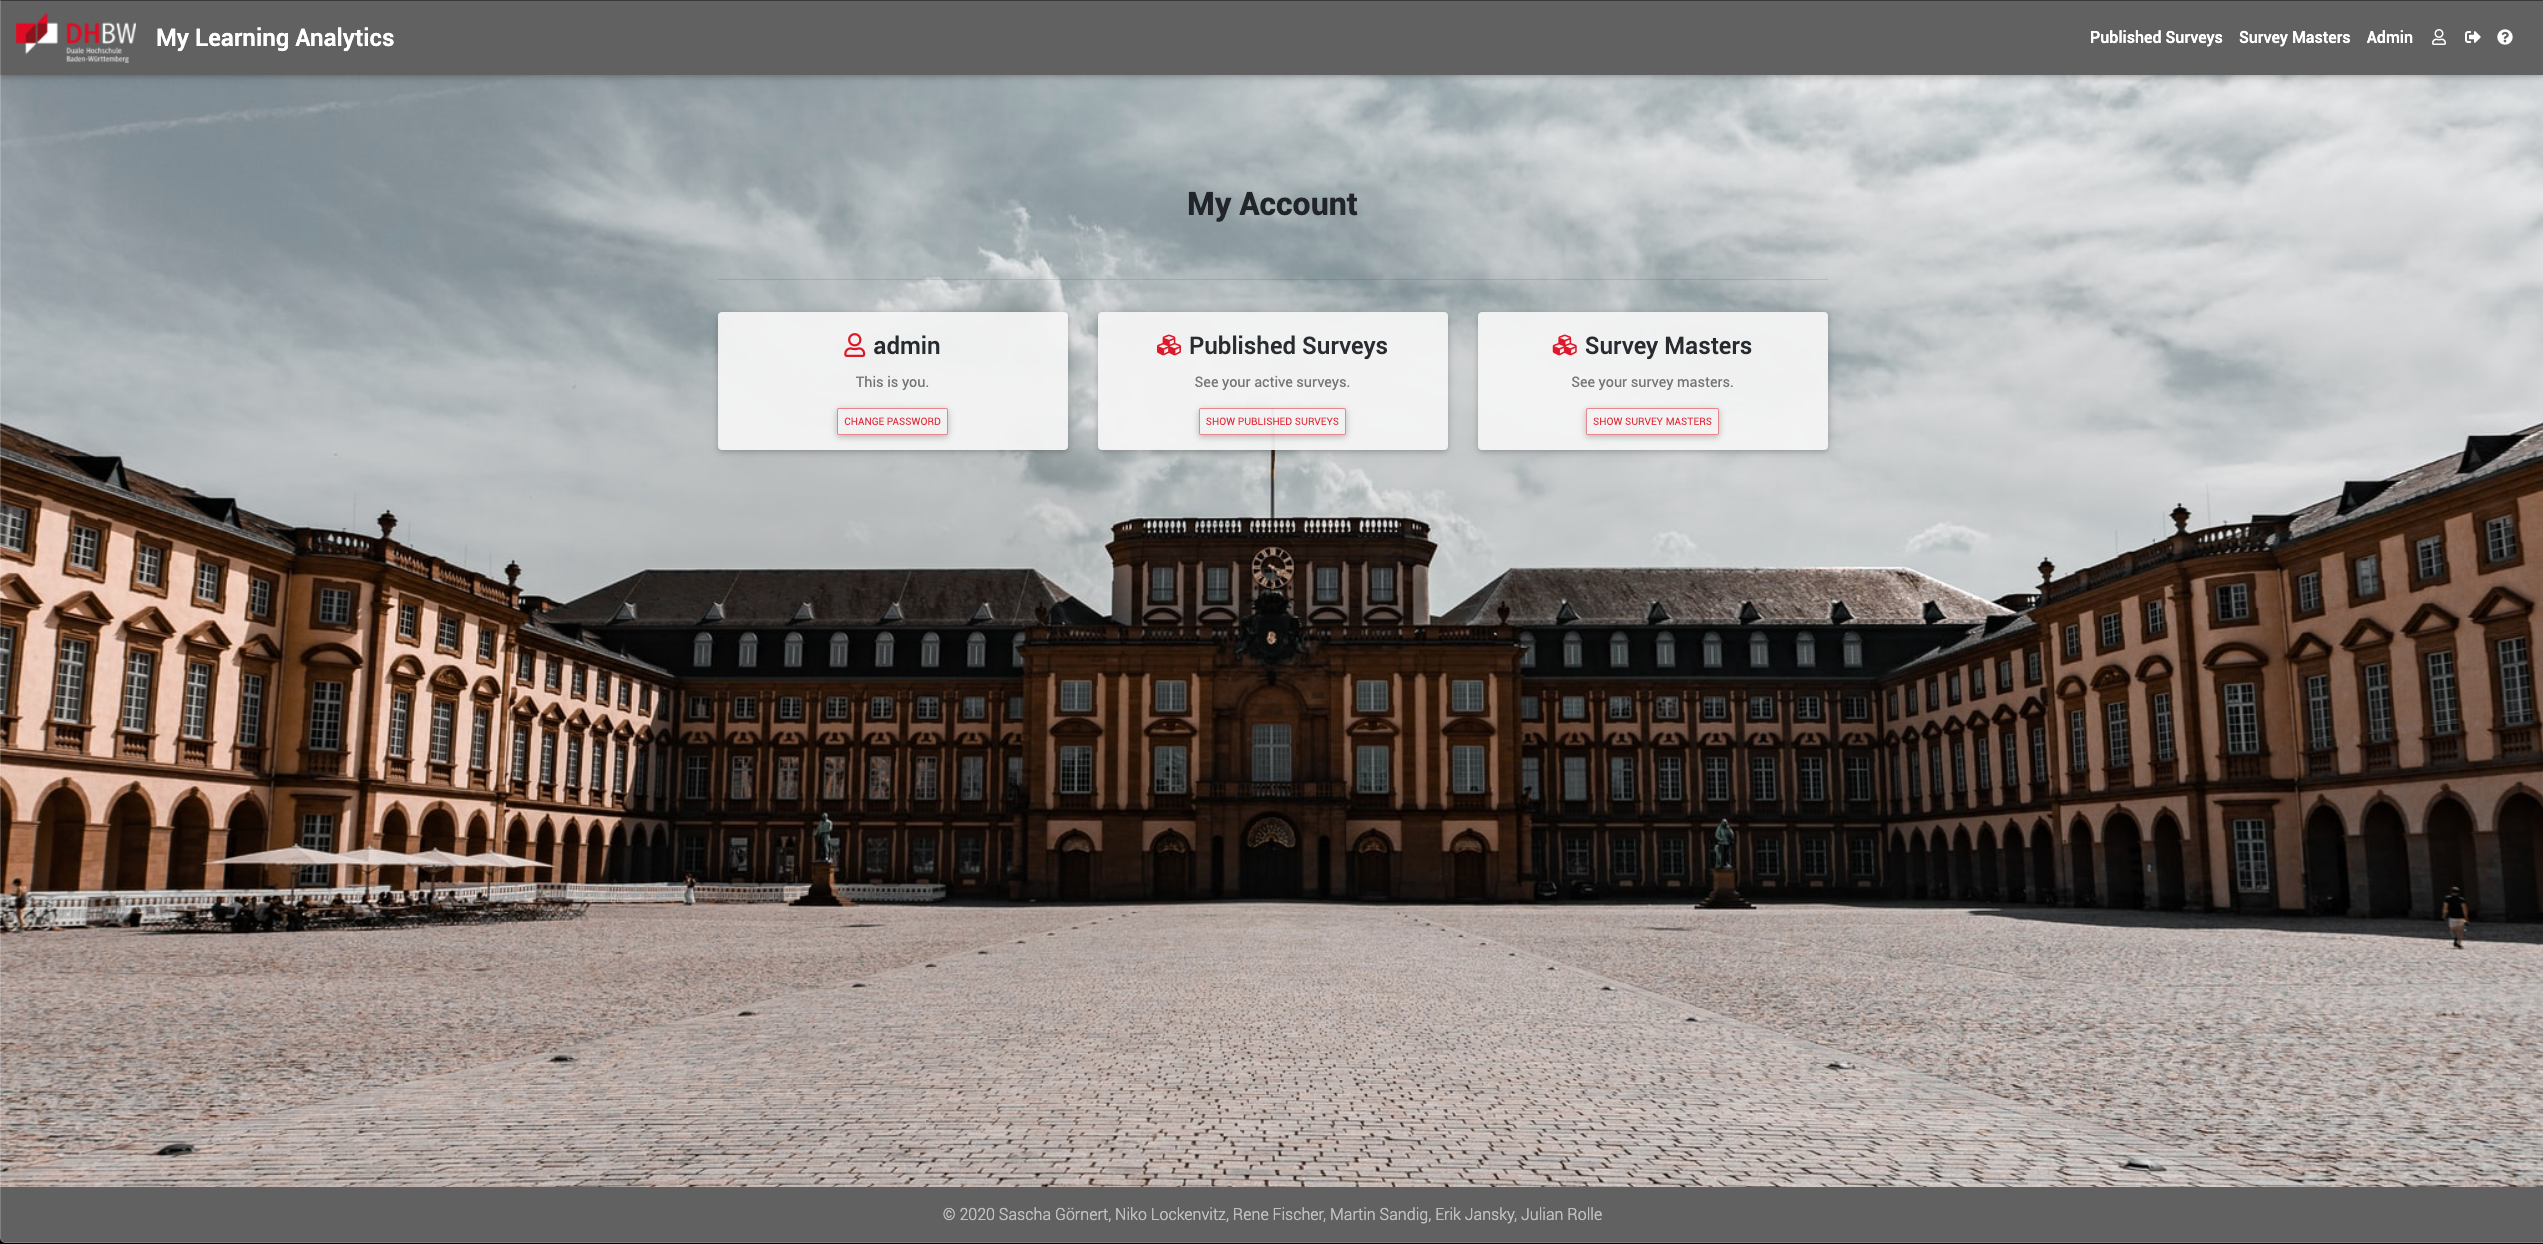
\includegraphics[width=0.95\textwidth, keepaspectratio]{img/client/Account.png}
	\captionsetup{justification=centering, format=plain}
	\caption[\acl{UI}: Benutzerkonto]{\acl{UI}: Benutzerkonto \\ \quelleScreenshot}
	\label{fig:AccountImplement}
\end{figure}
